%
% File acl2014.tex
%
% Contact: giovanni.colavizza@epfl.ch
%%
%% Based on the style files for ACL-2013, which were, in turn,
%% Based on the style files for ACL-2012, which were, in turn,
%% based on the style files for ACL-2011, which were, in turn, 
%% based on the style files for ACL-2010, which were, in turn, 
%% based on the style files for ACL-IJCNLP-2009, which were, in turn,
%% based on the style files for EACL-2009 and IJCNLP-2008...

%% Based on the style files for EACL 2006 by 
%%e.agirre@ehu.es or Sergi.Balari@uab.es
%% and that of ACL 08 by Joakim Nivre and Noah Smith

\documentclass[11pt]{article}
\usepackage{acl2014}
\usepackage{times}
\usepackage{url}
\usepackage{latexsym}
\usepackage[urlbordercolor={1 1 1}]{hyperref}
\usepackage[color=green]{todonotes}
\newcommand{\code}[1]{\texttt{#1}}

\usepackage{amsmath}
\usepackage{amssymb} %for the curvy L
\usepackage{subcaption} %for, well, subcaption
\usepackage{booktabs}

\usepackage[autocite=inline, maxnames=2, minnames=1, style=authoryear]{biblatex}
\addbibresource{refs.bib}

\usepackage{multicol}

\usepackage{adjustbox}
\widowpenalty = 1000
\clubpenalty = 1000

\title{Topic analysis of online newspapers}

\author{
  Jean-Marc Bejjani \\
  \And
  Luca Montanelli \\\\
  {\tt \{jean.bejjani,luca.montanelli,christophe.muller\}@epfl.ch} 
  \And
  Christophe Muller \\
  }

\date{December 16th, 2018}

\begin{document}
\maketitle

\begin{abstract}
The NOW corpus contains numerous articles from english speaking countries. We begin by optimizing the process to create LDA model for this database. Then with the said model we can interestingly classify the different countries according to their similarity media-wise and observe the main topics of importance in typical representatives of those classes. We end the study with the observation of the time evolution of the discovered topics.
\end{abstract}



\section{Introduction}
The goal of our project is to use machine learning techniques in order to get a better understanding of how information is shared around the world. Information is dynamic and evolves with time and culture. Analyzing these changes can help us develop a critical opinion regarding the origin of a given piece of information.

Our approach consists in creating a topic model of newspaper articles.
LDA (Latent Dirichlet Allocation) will be used for the topic modelling, with a list of word as input it will give us extracted topics as a probability distribution of words. This way each article has an associated topic distribution and each topic has a given word distribution. 

This assignation of topics to articles should allow us to give an insight as to which country is more or less oriented in specific topics. In the best scenario we hope to see a topic becoming more present after specific large scale events and observe more coverage of some topics worldwide in the case of an event with global impact.


\section{Dataset}
The dataset this work is based on is the \href{https://corpus.byu.edu/now/}{\textit{News On the Web} (NOW) corpus}.
A sample of the dataset available on the website was used to test the data processing steps, then since all the data ranging from January 2010 to October 2016 was available on the ADA cluster we didn't need to scrap data from somewhere else. To use optimally the cluster's resources, all data treatment operations were performed with the \code{pyspark} library.

\subsection{Data description}
This corpus consists in a database of online articles from 20 english-speaking countries, it represents nearly 5.3 million articles containing more than 6.9 billion words as of now. The dataset is made of \code{.txt} files with the information separated in several types of files.
Two of these are particularly useful in our study: the \code{sources.txt} and the \code{wlp.txt}.
The \code{sources.txt} contains a list of all articles with unique text ID, title, author, date, count of words, source newspaper and link to the source.
There is a \code{wlp.txt} for each month for each country. One of these files contains the full articles of the month of the given country. In it, each \textit{word} of the text is associated with a \textit{lemma} (linking the word to its canonical form) and a \textit{part of speech} (PoS, giving information on the use of the word in the sentence). Furthermore, all wlp combinations have an associated text ID which makes it very easy to link them to their text information.

Among the other (less important) files we find a \code{lexicon.txt} listing all words found in the dataset and their corresponding lemmas and the \code{text.txt} files containing the complete text of every article.

\section{Methods}

\subsection{Data pre-processing}
The LDA model needs a list of significant words as input to output meaningful topics, we need to avoid the `garbage in - garbage out' phenomenon.
All numbers, punctuation, foreign-language, unimportant proper nouns are easily filtered with their respective \textit{part of speech}.
We use a comprehensive list of `stopwords' to filter the most common words in the English language (`the', `be', `and', etc).
To keep a list of lemmas which will more likely give a significant topic modelling we also need to filter the least and most common lemmas. Therefore, we scrape the top 1\% of all the lemmas and keep only those which appear in more than 200 documents. Consequently, out of the roughly 600'000 unique lemmas that are kept after filtering PoS and stopwords, we end up with 50'000 which we will use in our model.

\subsection{Text representation}
After filtering and grouping by text, we are left with a dataframe containing a list of important words for each text. From there, we apply a `tfidf' transformation which we then normalize for each document. The tfidf matrix is an advanced bag-of-words (bow) representation which will scale words according to how much they are used in the whole corpus. Normalization is very important because models are sensible to difference in scales. Here, a longer text will obviously contain more words and thus its associated bow vector will be longer. Normalization therefore prevents the model to be skewed towards longer articles.

\subsection{LDA model and hyperparameters}
In LDA, documents are assumed to be probability distributions over topics which are in turn distributions over all the words in the corpus. It is important to note that LDA does not take into account the order of the words, documents are just bags where words are thrown in with a different probability each. It is possible to do so to a certain extent if using bi- or trigrams.

Formally, we can define a few variables that LDA uses:
\begin{itemize}
    \item $\theta_{m}$ is the topic distribution for document m
    \item $Z_{mn}$ is the topic for the n-th word of the m-th document
    \item $\varphi_{k}$ is the word distribution for topic $K$
    \item $W_{mn}$ is the n-th word of the m-th document
\end{itemize}

\begin{figure}[htpb!]
    \centering
    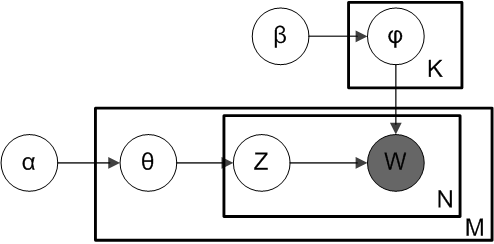
\includegraphics[width=.4\textwidth]{images/LDA.png}
    \caption{Plate notation for LDA model.}
    \label{fig:lda}
\end{figure}

Figure \ref{fig:lda} shows the plate notation for a typical LDA model. LDA has three hyperparameters that we can tune, these are:
\begin{itemize}
    \item $K$ the number of topics
    \item $\alpha$ the prior over topic distribution for documents
    \item $\beta$ the prior over word distribution for topics
\end{itemize}

In practice, a big $\alpha$ means that documents are likely to be represented by a high number of topics and vice versa. Similarly, a high $\beta$ will mean that topics will be composed of many words. 

\subsection{Model tuning}
For our case, with texts coming from media outlets, we want to concentrate on a few major topics such as politics, economics, cooking, sports, etc... We want to prevent excessively fine topics such as `Brexit', `Trump', `Football' or `Curry' which will be very localized. As a result, we also want topics to encompass many words. This means that we will be using a small $\alpha$ while using a big $\beta$.

Although unsupervised, LDA models have metrics to score them. One such metric is the perplexity which is a decreasing function of the log-likelihood ($\mathcal{L}(w)$):

\begin{equation*}
    \textrm{Perplexity} = \exp\left(\frac{\mathcal{L}(w)}{W}\right)
\end{equation*}

The lower the perplexity, the better. With this we could then score the perplexity (or log-perplexity with spark) on a held-out test set which would enable us to use cross-validation to choose the best hyperparameters within an acceptable range. 

However, perplexity gives us a few problems. First of all, it is always going to be minimized with a higher number of topics. This means that it is a bad metric here where we want to stay with few topics. Furthermore, perplexity is weakly anti correlated to how human perceive topics \autocite{Cha:09}, which is the reason we decided to not use it in our hyperparameter search. Instead, we ran locally (on a sample of the data) different LDA models and then subjectively judged the results ourselves.


For the exact values of $\alpha$ and $\beta$, Griffiths (\citeyear{Gri:04}) suggests $\frac{50}{K}$ and 0.1 respectively with $K$ the number of topics. Our search found that $\frac{10}{K}$ and $\frac{1}{K}$ provided the best results. In addition to that, it was shown that using an asymmetric $\alpha$ and a symmetric $\beta$ outperformed any other combination \autocite{Wal:09}. Thus we use, for $K=10$, an asymmetric $\alpha$ of $\frac{1}{k}$ with small $k$ the index of a topic. Once we had the hyperparameters, we tested on the cluster with a fraction of the data and found that ten topics made the most sense. 5 topics lead to good ones but they seemed to overlap (see fig.~\ref{fig:topicsa}), and 15 generated topics which did not make sense (fig.~\ref{fig:topicsb}). 

\begin{figure}[htpb!]
  \begin{subfigure}[t]{.45\linewidth}
    \centering
    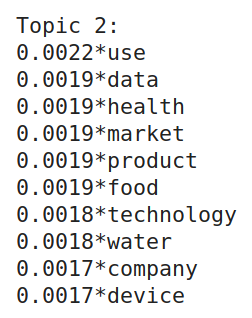
\includegraphics[height=1\linewidth]{images/K=5.png}
    \caption{Bad topic with K=5 where health, economics and technology seem to mix}
    \label{fig:topicsa}
  \end{subfigure}
  \hfill
  \begin{subfigure}[t]{.45\linewidth}
    \centering
    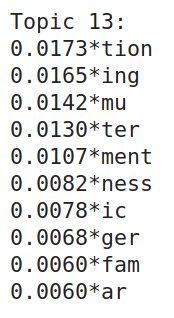
\includegraphics[height=1\linewidth]{images/K=15.png}
    \caption{Nonsensical topic with K=15}
    \label{fig:topicsb}
  \end{subfigure}
  \caption{Examples of bad topics due to too low and too high number of topics.}
  \label{fig:topics}
\end{figure}

Another very important aspect of the spark LDA is the number of iterations it performs. We have seen that this is the foremost parameter to modify and has the greatest impact. Our models ran with 1000 iterations because even 750 did not provide topics good enough.

In conclusion, we performed LDA with ten topics using an asymmetric $\alpha$ of $\frac{1}{k}$ with online optimisation and a symmetric $\beta$ of 0.1.

\section{Results}

The topic distribution for all the articles gave to our data points low dimensionality we can exploit to perform analysis and get interesting results.
The ten topics discovered by our LDA model are described in Table~\ref{tab:topics} (in appendix) with the first five words they contain. We easily inferred each topic title from the words that make them: Law, transport, food, economics, sport, technology, health, nature (\& science), politics and entertainment.



\subsection{Geographical analysis}

We wanted to observe how different countries can have similar topic distributions and if their similarities can correlate to their cultural background and geographic location. 

\subsubsection{Clustering of countries}

We started by clustering the countries using K-mean using the 10 topics as dimensions. This was done after averaging the topics values of all articles for each country. Then in order to visualize our results we performed PCA to reduce the dimensions to 2. 
This allowed us to group the countries into 5 groups with similar topic distributions and observe if they are close culturally and geographically.

\begin{figure}[hbtp!]
    \centering
    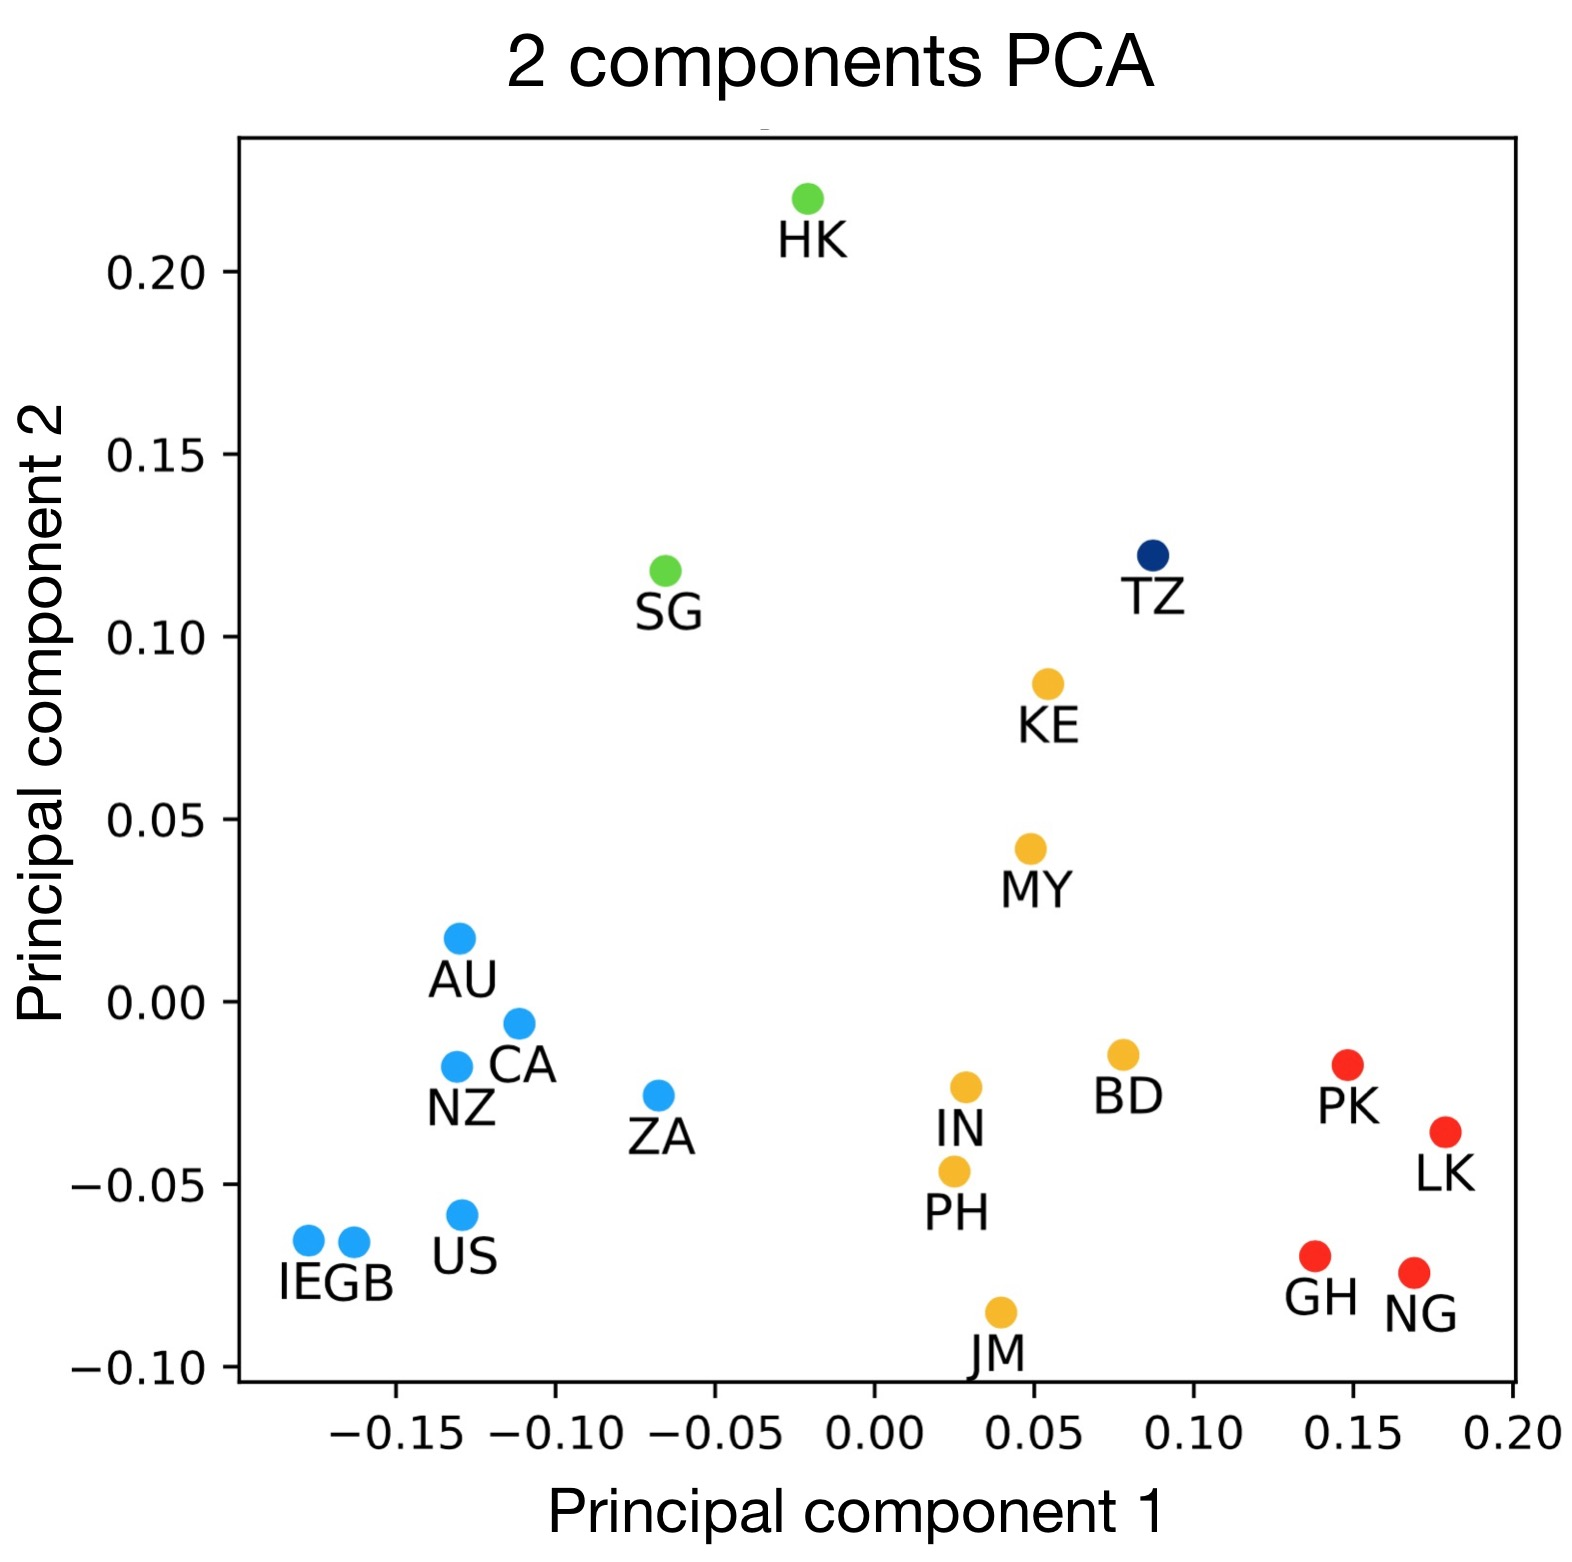
\includegraphics[width=.9\linewidth]{images/pca.jpg}
    \caption{PCA projection of the 20 countries}
    \label{fig:pca}
\end{figure}

As we can see in Figure~\ref{fig:pca} the countries in each group share a similar cultural and/or an economic background. The groups we observe are the following:
\begin{itemize}
    \item Light blue: western countries or countries with strong western influence. ex: Australia, Canada, United States, Great Britain, etc.
    \item Green: Asian city-states with strong economy. ex: Hong Kong and Singapore.
    \item Yellow: Developing countries in South-Asia or Africa. ex: India, Kenya, etc.
    \item Red: Another group of developing countries in South-Asia or Africa. ex: Pakistan, Nigeria, etc.
    \item Dark blue: Tanzania.
\end{itemize}

This classification is very useful in order to asses how similar certain countries are in term of newspaper content.



\subsubsection{Topic distribution analysis}
In Figure~\ref{fig:5countries} we observe the relative importance of each topic in one country from each of the five groups: USA, Hong Kong, India, Nigeria and Tanzania.
Among the points standing out from the rest we may observe and deduce events or general trends. In economics Hong Kong is obviously dominant given its strong corporate and financial driven economy, it is also second place in technology behind Tanzania which we don't explain.
The entertainment sector seems dominated by the USA and India, this is only natural knowing that Hollywood and Bollywood have a big impact in the local media (and abroad).
In politics Nigeria stands out from the rest quite significantly, we expected a lot more from the USA but compared to the numerous \textit{coup d'etat} in Nigeria \autocite{bbc:18} and the more eventful elections in India and Tanzania it is understandable to have these countries with a less `standard democracy' talk a lot about politics.

Overall we observe that in the USA (similarly to the countries in the same group see fig.~\ref{fig:pca}) topics are more uniformly covered in the press compared to the rest of the world.

\begin{figure}[hbtp!]
    \centering
    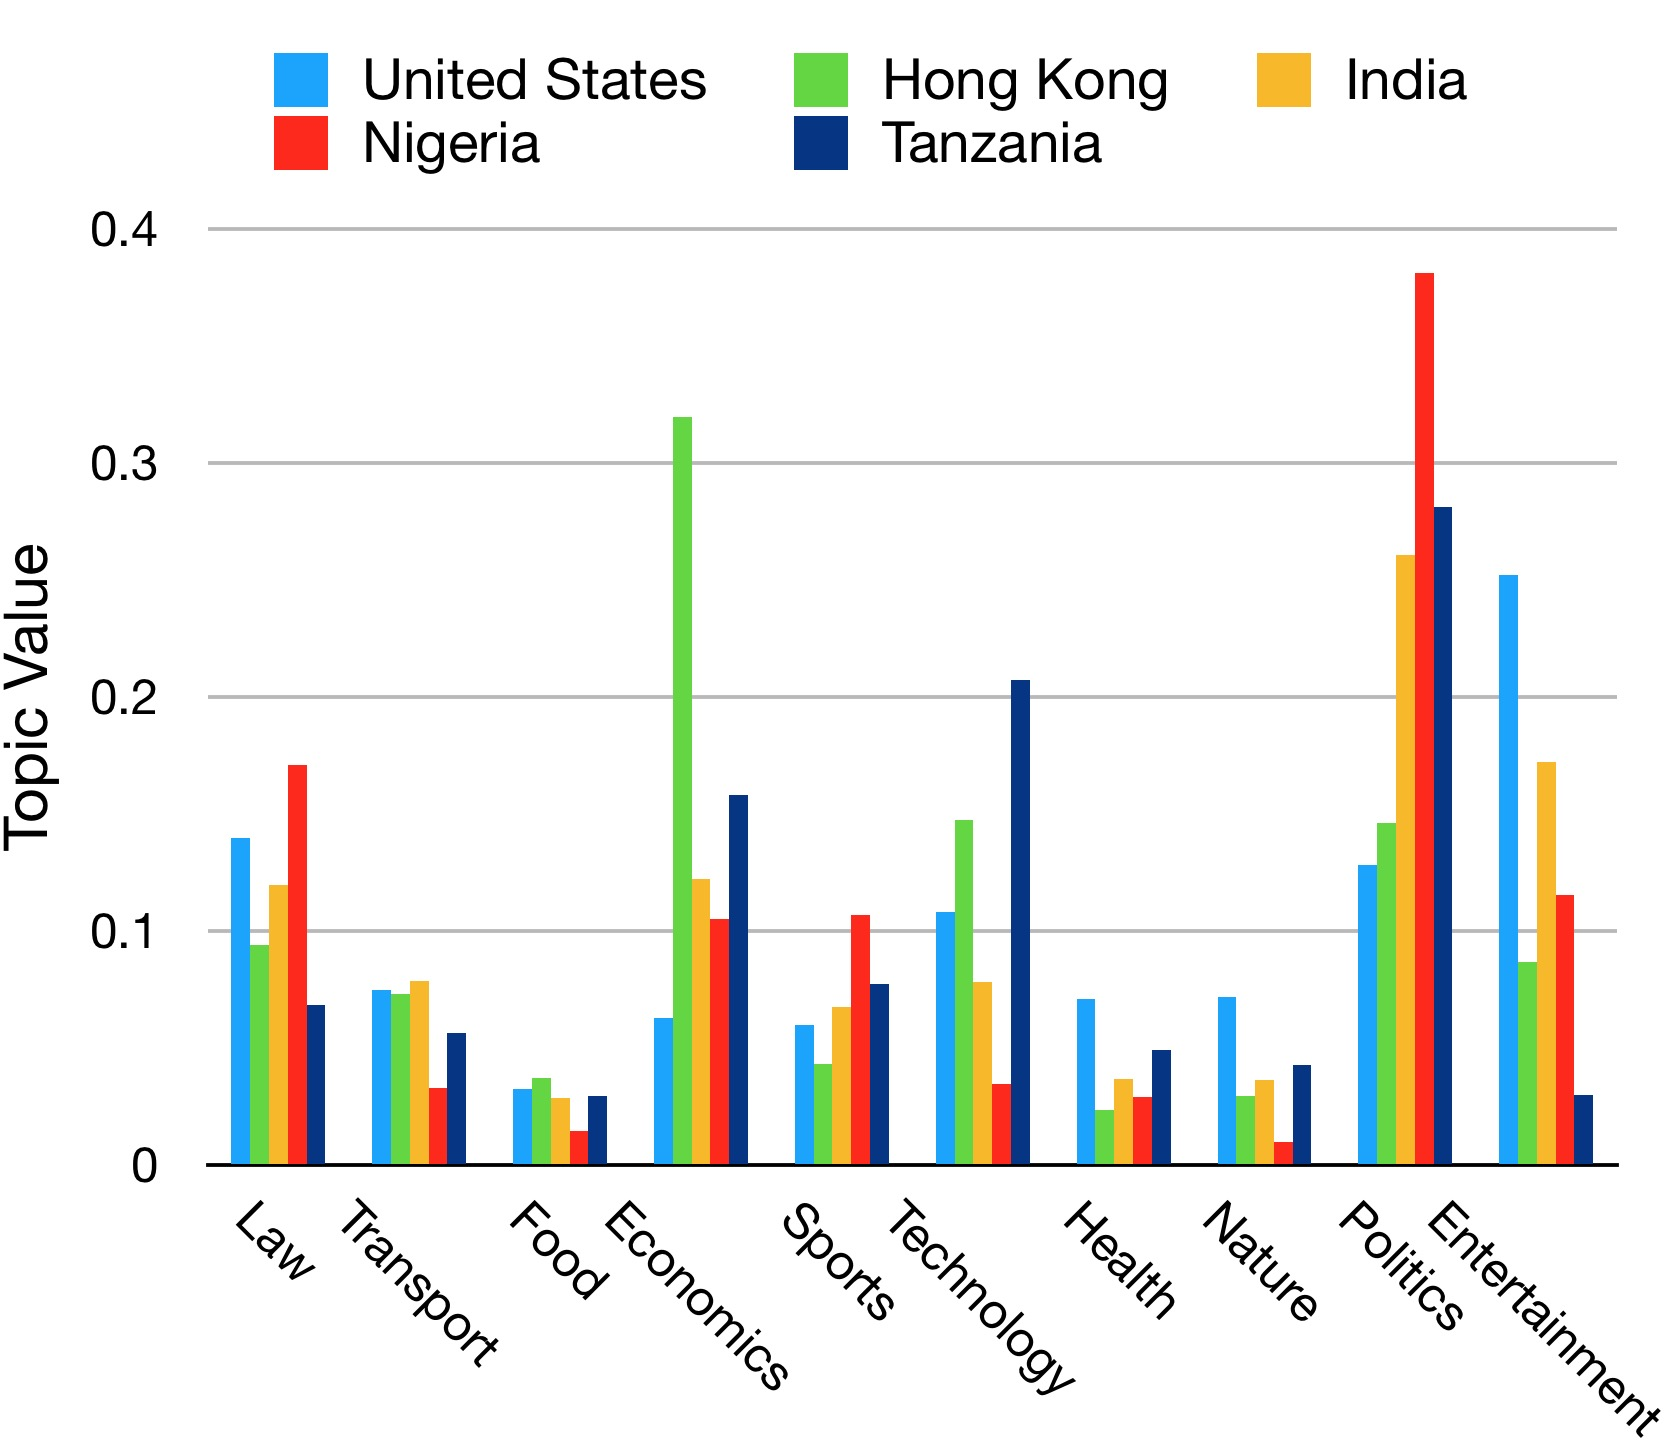
\includegraphics[width=\linewidth]{images/5countries.jpg}
    \caption{Topic importance in 5 countries}
    \label{fig:5countries}
\end{figure}


\subsection{Observations through time}
We observe different behaviours depending on the topic when looking at the variations in time. Some have little to no change while others show big variations and even (inversely-) correlated evolution.

In Figure~\ref{fig:2topics} we look at the evolution of politics versus entertainment and observe some inverse correlation between the two topics, indicatively, the Pearson correlation coefficient equals $-0.95$. It is important to note that these observations are on a worldwide level and cannot be attributed to a single country. Nevertheless we observe a clear tendency of politics becoming more present in the media as opposed to `fun' subjects like entertainment. This may or may not be linked to the start of the migrant crisis in Europe and the numerous ISIS terror attacks worldwide.
\begin{figure}[htbp!]
    \centering
    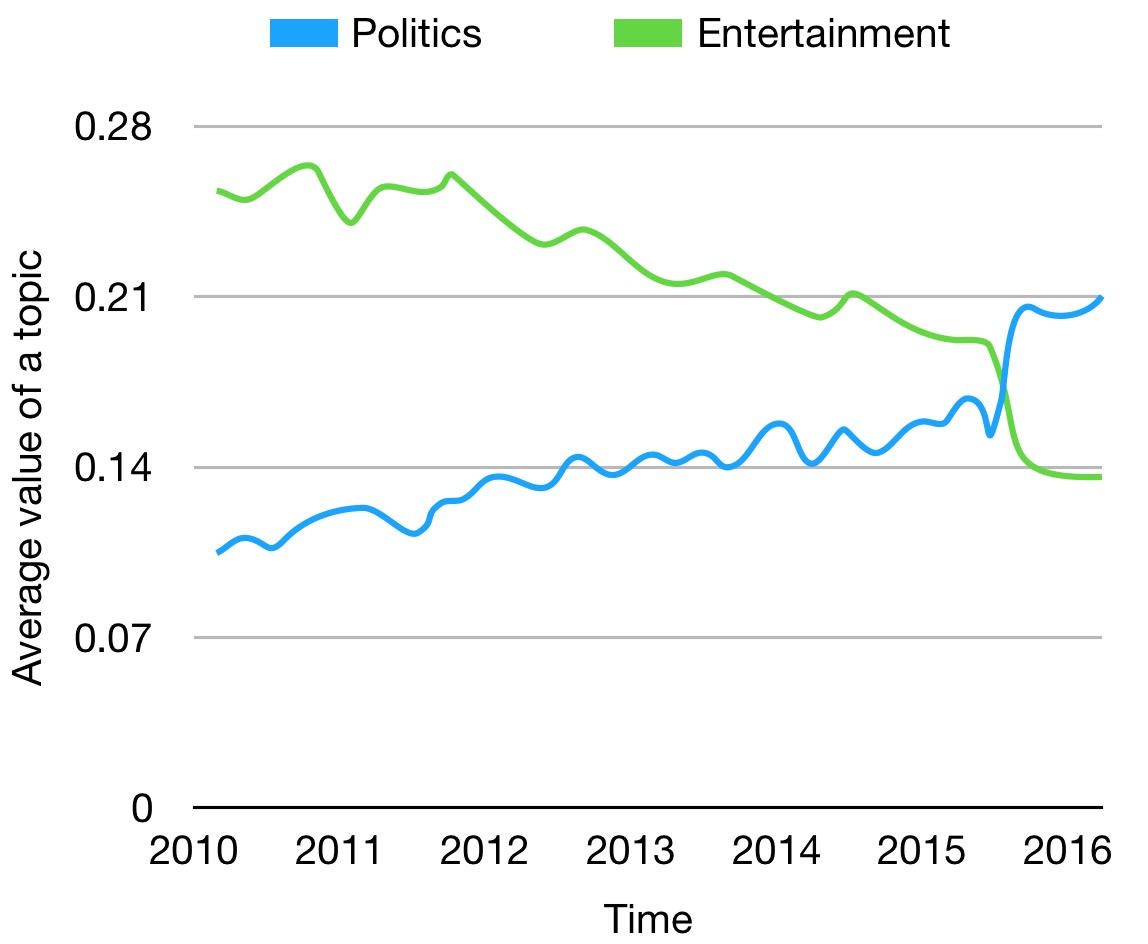
\includegraphics[width=\linewidth]{images/polandent.jpg}
    \caption{Variation of politics \& entertainment}
    \label{fig:2topics}
\end{figure}

Conversely in Figure \ref{fig:5topics} we see the evolution of five topics (nature, health, food, technology, transport) which don't seem to undergo any major change. This is understandable given the `neutral' nature of these topics.

\begin{figure}[htbp!]
    \centering
    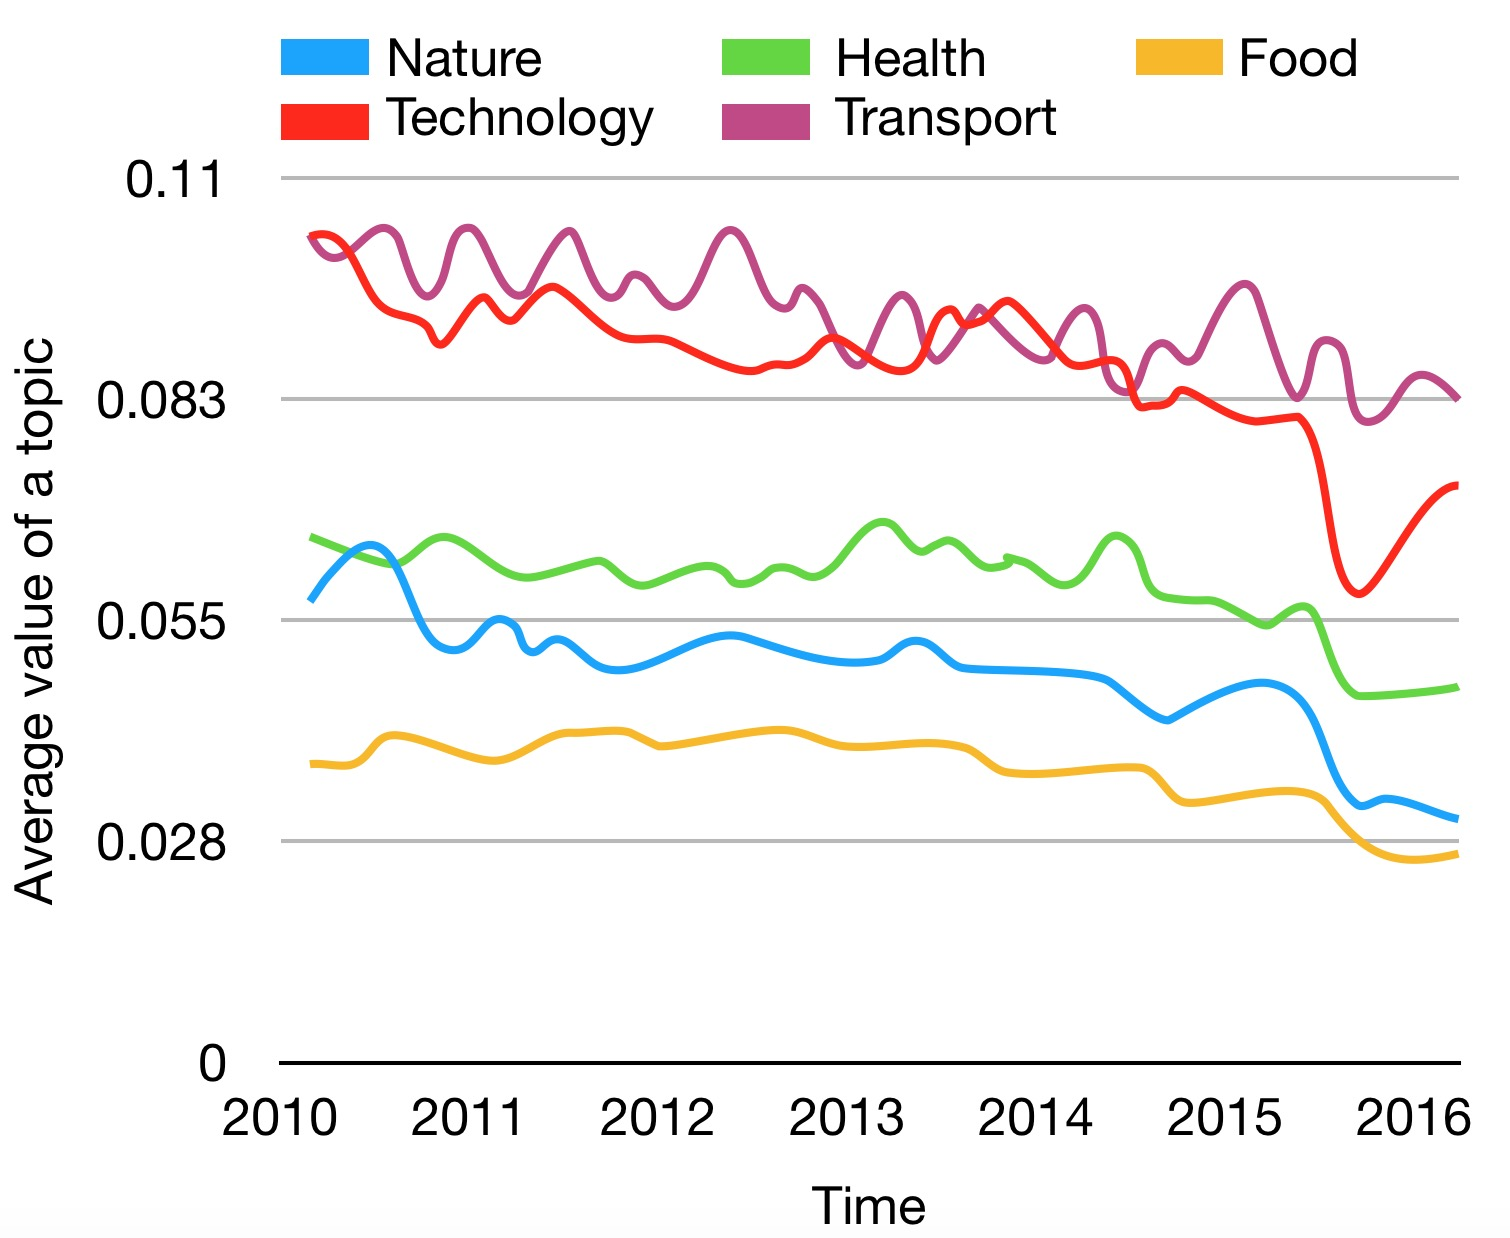
\includegraphics[width=\linewidth]{images/stagningtopics.jpg}
    \caption{Five topics with weak variations, the scale is smaller than on figure \ref{fig:2topics}.}
    \label{fig:5topics}
\end{figure}


\onecolumn

\begin{multicols}{2}

\section{Conclusion}

In this project we managed to extract valuable information from a large dataset of articles and analyze it in a geographical and socio-economical context. Topic modeling is a powerful tool for reducing dimensions for large sets of text based data. This can be used to perform a lot of different analysis of the data and the approach we took in this project is just one of them.

Some things we could improve in our model are applying a better pre-processing as we can see that in \ref{fig:topics} we sometimes get nonsensical topics. This would allow us to have a larger number of more specific topic and study their evolution in time and space. We could also try to balance out the training data between the different countries to avoid biases.\vfill

\nocite{*}
\printbibliography[]

\end{multicols}

\bigskip
\section*{Appendix}

\begin{table}[htbp!]

\centering%useless
\caption{The 10 topics obtained with LDA}
\label{tab:topics}

%\begin{adjustbox}{angle=270}

\begin{tabular}{@{}lrrrrr@{}}
\toprule
\multicolumn{1}{l}{Topic name} & \multicolumn{5}{c}{Five most significant words per topic} \\
\cmidrule(r){1-1}\cmidrule(l){2-6}
Law : & police & court & arrest & charge & officer \\
Transport : & car & road & city & building & vehicle \\
Food : & food & farmer & restaurant & wine & fruit \\
Economics : & company & bank & price & market & cent \\
Sport : & game & player & team & win & league \\
Technology : & company & technology & business & market & customer \\
Health : & health & patient & cookie & hospital & cancer \\
Nature : & water & animal & climate & species & plant \\
Politics : & government & party & minister & student & state \\
Entertainment : & film & music & movie & show & life \\ \bottomrule
\end{tabular}

%\end{adjustbox}

\end{table}

\end{document}
